\documentclass[10pt,graphicx,caption,rotating]{article}
\textheight=24cm
\textwidth=18cm
\topmargin=-2cm
\oddsidemargin=0cm
\usepackage[utf8x]{inputenc}
\usepackage[activeacute,spanish]{babel}
\usepackage{amssymb,amsfonts}
\usepackage[tbtags]{amsmath}
\usepackage{slashbox}
\usepackage{pict2e}
\usepackage{float}
\usepackage[all]{xy}
\usepackage{graphics,graphicx,color,colortbl}
\usepackage{times}
\usepackage{subfigure}
\usepackage{wrapfig}
\usepackage{multicol}
\usepackage{cite}
\usepackage{url}
\usepackage[tbtags]{amsmath}
\usepackage{amsmath,amssymb,amsfonts,amsbsy}
\usepackage{bm}
\usepackage{algorithm}
\usepackage{algorithmic}
\usepackage[centerlast, small]{caption}
\usepackage[colorlinks=true, citecolor=blue, linkcolor=blue, urlcolor=blue,
breaklinks=true]{hyperref}

\begin{document}
\title{\Huge {Amplificadores Simples con BJT's}}
\author{Jose Duarte Código: $260983$\\
	David Ricardo Martínez Hernández Código: $261931$\\
	 Código: $ $}
\date{}
\maketitle
\floatname{algorithm}{Algoritmo}

\section{Materiales}
\begin{itemize}
 \item Cables y Conectores
 \item Fuente D.C
 \item Generador de Señales
 \item Multímetro
 \item Osciloscopio
 \item Pinzas
 \item Protoboard
 \item Resistencias
 \item Transistores BJT $2N3904$
\end{itemize}

\section{Procedimiento}
\noindent
\subsection{Emisor Común}
\begin{figure}[H]
	\centering
		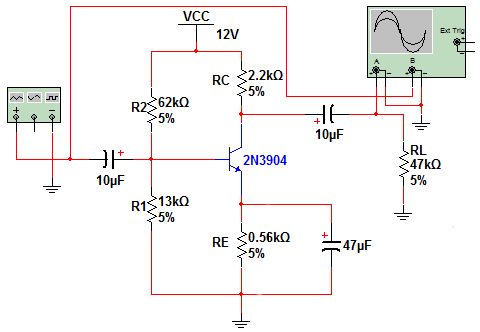
\includegraphics[scale=0.7]{emisor_comun.png}
	\caption{Circuito Emisor Común}
	\label{fig1}
\end{figure}
\noindent
Para la primera parte de laboratorio (Emisor común Figura \ref{fig1}), se utilizaron estas resistencias $R_C = 2.2$ K$\Omega$,  $R_E = 0.56$ K$\Omega$, $R_1 = 13$ K$\Omega$ y $R_2 = 62$ K$\Omega$. Al realizar las medidas de dichas resistencias con el multímetro se obtuvieron los siguientes resultados. Cuadro \ref{tab1}.
\begin{table}[H]
	\centering
\begin{tabular}[c]{|c||c|c|} \hline
Elemento & Valor Nominal & Valor Medido \\ \hline
$R_1$ & $13$ K$\Omega$ & $13.003$ K$\Omega$ \\ \hline
$R_2$ & $62$ K$\Omega$ & $61.52$ K$\Omega$ \\ \hline
$R_C$ & $2.2$ K$\Omega$ & $2.225$ K$\Omega$ \\ \hline
$R_E$ & $0.56$ K$\Omega$ & $0.5136$ K$\Omega$ \\ \hline
\end{tabular}
	\caption{Tabla de valores tomados para el montaje}
	\label{tab1}
\end{table}
\noindent
Los valores de operación del transistor fueron los siguientes
\begin{table}[H]
	\centering
\begin{tabular}[c]{|c||c|c|c|} \hline
 & Voltaje Teórico & Voltaje Práctico & \textbf{Error} \\ \hline
$V_E$ & $1.132$ V & $1.375$ V & $21\%$ \\ \hline
$V_B$ & $2.08$ V & $2.025$ V & $2.64\%$ \\ \hline
$V_C$ & $7.5494$ V & $7.01$ V & $7.14\%$ \\ \hline
$V_{CE}$ & $6.4124$ V & $5.653$ V & $7.63\%$ \\ \hline
\end{tabular}
	\caption{Tabla de valores tomados para el montaje en polarización}
	\label{tab2}
\end{table}
\noindent
La corriente de colector no se midió de manera directa, entonces se utiliza la ley de Ohm, dando como resultado $2.204$ mA, siendo muy similar al valor pedido en el diseño de $2.2$ mA.\\
Se realizaron 3 tomas de datos diferentes para el montaje de la Figura \ref{fig1}, medidos en $V_{RMS}$ cada uno consignados en el Cuadro \ref{tab3}
\begin{table}[H]
	\centering
\begin{tabular}[c]{|c|c|c|c|} \hline
$V_{IN}$ & $V_{OUT}$ & \textbf{Ganancia Práctica} V/V & \textbf{Error en la ganancia} \\ \hline
$8.64$ mV$_{RMS}$ & $1.02$ V$_{RMS}$ & $-118.056$ & $1.64\%$ \\ \hline
$8.94$ mV$_{RMS}$ & $1.07$ V$_{RMS}$ & $-119.687$ & $3.04\%$ \\ \hline
$9.53$ mV$_{RMS}$ & $1.13$ V$_{RMS}$ & $-118.573$ & $2.08\%$ \\ \hline
\end{tabular}
	\caption{Tabla de valores tomados para el montaje en pequeña señal}
	\label{tab3}
\end{table}
\noindent
Siendo la ganancia teórica de $-116.148$ V/V.\\
El límite de la banda media (magnitud de $1.13$ V$*1/ \sqrt{3}=0.798$ V)  a una frecuencia de $375.4$ Hz, por debajo de la frecuencia medida inicialmente, al subir la frecuencia no varío la magnitud de la salida con las frecuencias que daba el generador.\\
Al desconectar el condensador de desacople de $47\ \ \mu$F y al aumentar la entrada se observo que la señal no se amplificaba mucho (Cuadro \ref{tab4})
\begin{table}[H]
	\centering
\begin{tabular}[c]{|c|c|c|} \hline
$V_{IN}$ & $V_{OUT}$ & \textbf{Ganancia Práctica} V/V \\ \hline
$42.7$ mV$_{RMS}$ & $109$ mV$_{RMS}$ & $-2.55269$ \\ \hline
\end{tabular}
	\caption{Tabla de valores tomados para el montaje en pequeña señal sin condensador de desacople}
	\label{tab4}
\end{table}
\noindent
La impedancia de entrada del amplificador fue de $2.39266$ K$\Omega$. La inversión de fase se debe a que al aumentar la tensión de base, disminuye la tensión de salida, al disminuir la tensión de base, aumenta la tensión de salida, además la fuente de corriente establecida por el modelo de transconductancia la fuente de corriente dependiente se encuentra en sentido opuesto a la salida de tensión, esto genera la inversión de fase.\\
Al desconectar el condensador de desacoplo de emisor sucedió una caída de tensión, esto se debe a que se perdió la configuración de amplificador de emisor común y se transformo en un amplificador con degeneración.

\subsection{Base Común}
\begin{figure}[H]
	\centering
		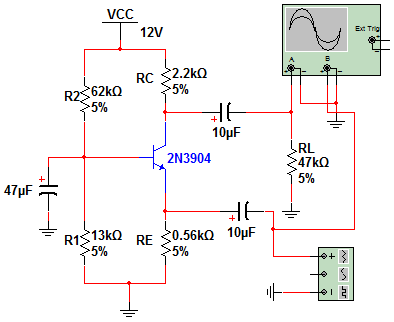
\includegraphics[scale=0.7]{base_comun.png}
	\caption{Circuito Base Común}
	\label{fig2}
\end{figure}
\noindent
Se utilizaron las mismas resistencias que en el montaje de la Figura \ref{fig1}, consignadas en el Cuadro \ref{tab1}.\\
Al realizar la medida del transistor en su punto de operación se obtuvieron los resultados consignados en el Cuadro \ref{tab3}.\\
\noindent
La corriente de colector no se midió de manera directa, entonces se utiliza la ley de Ohm, dando como resultado $2.204$ mA, siendo muy similar al valor pedido en el diseño de $2.2$ mA.\\
Se realizaron 3 tomas de datos diferentes para el montaje de la Figura \ref{fig2}, medida en $V_{RMS}$ cada uno consignados en el Cuadro \ref{tab6}
\begin{table}[H]
	\centering
\begin{tabular}[c]{|c|c|c|c|} \hline
$V_{IN}$ & $V_{OUT}$ & \textbf{Ganancia Práctica} V/V & \textbf{Error en la ganancia} \\ \hline
$10.1$ mV$_{RMS}$ & $50.05$ mV$_{RMS}$ & $25.50$ & $6\%$ \\
 \hline
\end{tabular}
	\caption{Tabla de valores tomados para el montaje en pequeña señal}
	\label{tab6}
\end{table}
\noindent
Siendo la ganancia teórica de $24.06$ V/V.\\
para 462 mV de entrada dan 446 mV de salida a 10 kHz.\\
Al desconectar el condensador de desacople de $47\ \ \mu$F y al aumentar la entrada se cae el voltaje porque la configuración del transistor ha cambiado y se transformó en una configuración con degeneración.\\
La impedancia de entrada del amplificador fue de $61.11$ $\Omega$. La inversión de fase se debe al mismo fenómeno que sucede en el amplificador de emisor común.\\

\subsection{Colector Común}
\begin{figure}[H]
	\centering
		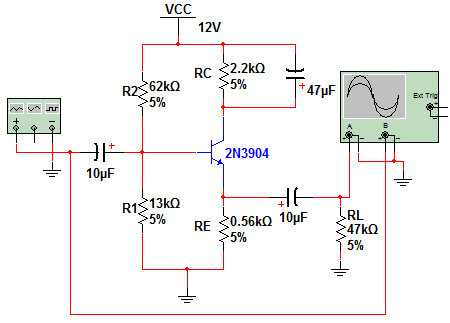
\includegraphics[scale=0.7]{colector_comun.png}
	\caption{Circuito Colector Común}
	\label{fig3}
\end{figure}
\noindent
Al igual que en el Base común se utilizaron las mismas resistencias iniciales del Cuadro \ref{tab1}.\\
Al realizar la medida del transistor en su punto de operación se obtuvieron los resultados consignados en el Cuadro \ref{tab3}.\\
\noindent
La corriente de colector no se midió de manera directa, entonces se utiliza la ley de Ohm, dando como resultado $2.204$ mA, siendo muy similar al valor pedido en el diseño de $2.2$ mA.\\
Se realizaron 3 tomas de datos diferentes para el montaje de la Figura \ref{fig3}, medidos en $V_{RMS}$ cada uno consignados en el Cuadro \ref{tab9}
\begin{table}[H]
	\centering
\begin{tabular}[c]{|c|c|c|c|} \hline
$V_{IN}$ & $V_{OUT}$ & \textbf{Ganancia Práctica V/V} & \textbf{Error en la ganancia} \\ \hline
$20$ mV$_{RMS}$ & $17$ V$_{RMS}$ & $0.946$ & $3\%$ \\ \hline
\end{tabular}
	\caption{Tabla de valores tomados para el montaje en pequeña señal}
	\label{tab9}
\end{table}
\noindent
Siendo la ganancia teórica de $0.976$ V/V.\\
El límite de la banda media (magnitud de $1.13$ V$*1/ \sqrt{3}=0.798$ V)  a una frecuencia de $375.4$ Hz, por debajo de la frecuencia medida inicialmente, al subir la frecuencia no varío la magnitud de la salida con las frecuencias que daba el generador.\\
La impedancia de entrada del amplificador fue de $9.89$ K$\Omega$. No hay inversión de fase en el amplificador de colector común.

\section{Conclusiones}
\noindent
\begin{itemize}
 \item Se conocieron las diferentes configuraciones para los BJT's, como lo es el emisor común que se utiliza para obtener ganancia de voltaje, el colector común que se utiliza para ganancia de corriente con una impedancia de entrada muy baja y para acople de impedancias, y finalmente el base común que se utiliza para amplificación de voltaje un poco más pequeña que el emisor común pero su ancho de banda es mas elevado.
 \item Las impedancias de cada amplificador son aprovechadas para realizar conexiones en cascada y así .
\end{itemize}

\bibliographystyle{ieeetran}
\begin{thebibliography}{99}
\bibitem{sedra} Jaeger, Richard C. \& Blalock, Travis N.
{\em "`Microelectronic Circuit Desing"'}.
McGraw-Hill, Fourth Edition, 1999.

\bibitem{sedra} Sedra, Adel S. \& Smith, Kenneth C.
{\em "`Circuitos Microelectrónicos"'}.
Oxford University Press, Cuarta Edición, 1999.
\end{thebibliography}
\end{document}